
\definecolor{c364fc7}{RGB}{54,79,199}
\definecolor{c5c940d}{RGB}{92,148,13}
\definecolor{c862e9c}{RGB}{134,46,156}
\definecolor{cc92a2a}{RGB}{201,42,42}


\def \globalscale {0.150000}
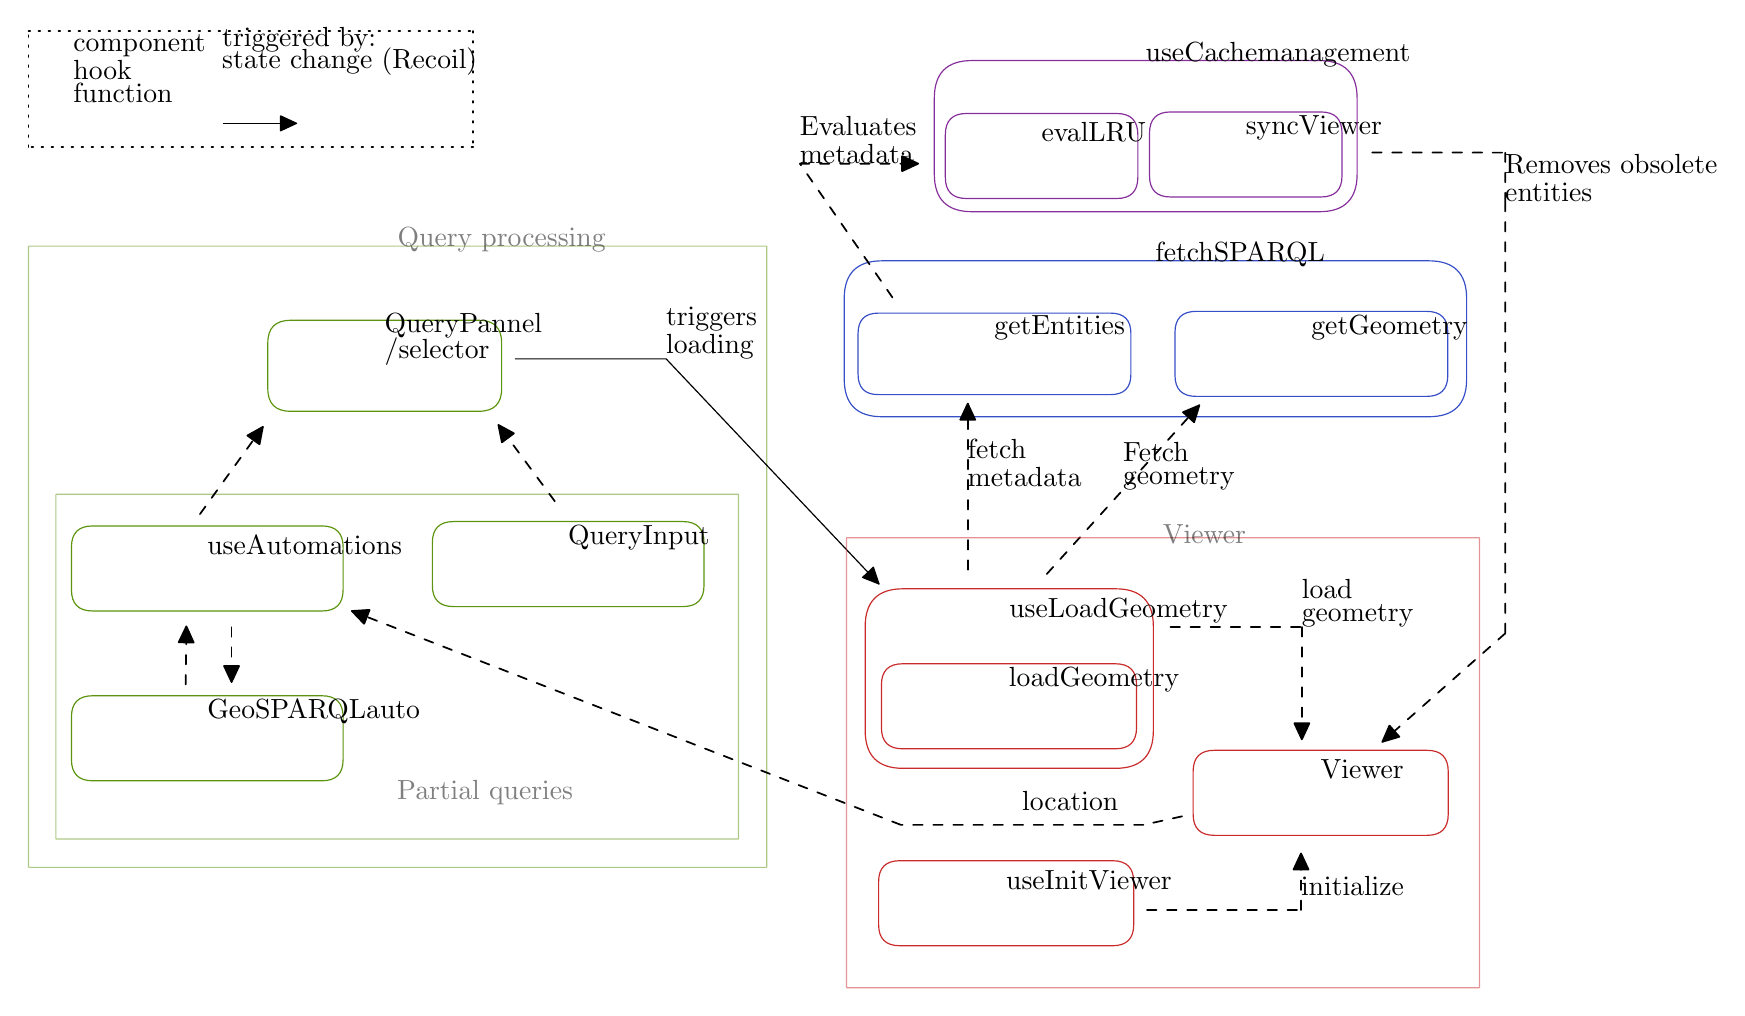
\begin{tikzpicture}[y=1cm, x=1cm, yscale=-\globalscale,xscale=\globalscale, inner sep=0pt, outer sep=0pt]
\begin{scope}[shift={(69.1386,19.532700000000002)},line cap=round]
  \path[draw=c364fc7,line width=0.015cm] (3.2000,0.0000)(3.2000,0.0000) ..
    controls (13.8000, 0.0000) and (24.4010, 0.0000) .. (49.5000,
    0.0000)(3.2000,0.0000) .. controls (12.5890, 0.0000) and (21.9780, 0.0000) ..
    (49.5000, 0.0000)(49.5000,0.0000) .. controls (51.6330, 0.0000) and (52.7000,
    1.0670) .. (52.7000, 3.2000)(49.5000,0.0000) .. controls (51.6330, 0.0000) and
    (52.7000, 1.0670) .. (52.7000, 3.2000)(52.7000,3.2000) .. controls (52.7000,
    5.3850) and (52.7000, 7.5690) .. (52.7000, 10.0000)(52.7000,3.2000) ..
    controls (52.7000, 4.6640) and (52.7000, 6.1270) .. (52.7000,
    10.0000)(52.7000,10.0000) .. controls (52.7000, 12.1330) and (51.6330,
    13.2000) .. (49.5000, 13.2000)(52.7000,10.0000) .. controls (52.7000, 12.1330)
    and (51.6330, 13.2000) .. (49.5000, 13.2000)(49.5000,13.2000) .. controls
    (32.5960, 13.2000) and (15.6920, 13.2000) .. (3.2000,
    13.2000)(49.5000,13.2000) .. controls (37.4150, 13.2000) and (25.3290,
    13.2000) .. (3.2000, 13.2000)(3.2000,13.2000) .. controls (1.0670, 13.2000)
    and (0.0000, 12.1330) .. (0.0000, 10.0000)(3.2000,13.2000) .. controls
    (1.0670, 13.2000) and (0.0000, 12.1330) .. (0.0000, 10.0000)(0.0000,10.0000)
    .. controls (0.0000, 8.2810) and (0.0000, 6.5620) .. (0.0000,
    3.2000)(0.0000,10.0000) .. controls (0.0000, 8.6030) and (0.0000, 7.2060) ..
    (0.0000, 3.2000)(0.0000,3.2000) .. controls (0.0000, 1.0670) and (1.0670,
    0.0000) .. (3.2000, 0.0000)(0.0000,3.2000) .. controls (0.0000, 1.0670) and
    (1.0670, 0.0000) .. (3.2000, 0.0000);



\end{scope}
\begin{scope}[shift={(89.0433,20.032700000000002)}]
  \path[fill=c364fc7] (6.4453,0.0000) node[above right] (text19){fetchSPARQL};



\end{scope}
\begin{scope}[shift={(0.075,18.2907)},fill opacity=0.500,draw opacity=0.500,line cap=round,transparency group]
  \path[draw=c5c940d,line width=0.015cm] (0.0000,0.0000) .. controls (14.3090,
    0.0000) and (28.6190, 0.0000) .. (62.5000, 0.0000)(0.0000,0.0000) .. controls
    (20.2630, 0.0000) and (40.5250, 0.0000) .. (62.5000, 0.0000)(62.5000,0.0000)
    .. controls (62.5000, 16.8980) and (62.5000, 33.7970) .. (62.5000,
    52.6000)(62.5000,0.0000) .. controls (62.5000, 18.0540) and (62.5000, 36.1070)
    .. (62.5000, 52.6000)(62.5000,52.6000) .. controls (39.6810, 52.6000) and
    (16.8630, 52.6000) .. (0.0000, 52.6000)(62.5000,52.6000) .. controls (49.5380,
    52.6000) and (36.5750, 52.6000) .. (0.0000, 52.6000)(0.0000,52.6000) ..
    controls (0.0000, 39.3050) and (0.0000, 26.0090) .. (0.0000,
    0.0000)(0.0000,52.6000) .. controls (0.0000, 34.7650) and (0.0000, 16.9310) ..
    (0.0000, 0.0000);



\end{scope}
\begin{scope}[shift={(21.950000000000003,18.790700000000005)},fill opacity=0.500,draw opacity=0.500,transparency group]
  \path[fill=c5c940d] (9.3750,0.0000) node[above right] (text27){Query
    processing};



\end{scope}
\begin{scope}[shift={(2.38912,39.2918)},fill opacity=0.500,draw opacity=0.500,line cap=round,transparency group]
  \path[draw=c5c940d,line width=0.015cm] (0.0000,0.0000) .. controls (13.2330,
    0.0000) and (26.4670, 0.0000) .. (57.8000, 0.0000)(0.0000,0.0000) .. controls
    (18.7390, 0.0000) and (37.4780, 0.0000) .. (57.8000, 0.0000)(57.8000,0.0000)
    .. controls (57.8000, 9.3810) and (57.8000, 18.7620) .. (57.8000,
    29.2000)(57.8000,0.0000) .. controls (57.8000, 10.0220) and (57.8000, 20.0440)
    .. (57.8000, 29.2000)(57.8000,29.2000) .. controls (36.6970, 29.2000) and
    (15.5940, 29.2000) .. (0.0000, 29.2000)(57.8000,29.2000) .. controls (45.8120,
    29.2000) and (33.8250, 29.2000) .. (0.0000, 29.2000)(0.0000,29.2000) ..
    controls (0.0000, 21.8190) and (0.0000, 14.4390) .. (0.0000,
    0.0000)(0.0000,29.2000) .. controls (0.0000, 19.2990) and (0.0000, 9.3990) ..
    (0.0000, 0.0000);



\end{scope}
\begin{scope}[shift={(22.5001,65.5918)},fill opacity=0.500,draw opacity=0.500,transparency group]
  \path[fill=c5c940d] (8.7891,0.0000) node[above right] (text35){Partial queries};



\end{scope}
\begin{scope}[shift={(3.70811,41.9804)},line cap=round]
  \path[draw=c5c940d,line width=0.015cm] (1.8000,0.0000)(1.8000,0.0000) ..
    controls (6.2420, 0.0000) and (10.6830, 0.0000) .. (21.2000,
    0.0000)(1.8000,0.0000) .. controls (5.7340, 0.0000) and (9.6680, 0.0000) ..
    (21.2000, 0.0000)(21.2000,0.0000) .. controls (22.4000, 0.0000) and (23.0000,
    0.6000) .. (23.0000, 1.8000)(21.2000,0.0000) .. controls (22.4000, 0.0000) and
    (23.0000, 0.6000) .. (23.0000, 1.8000)(23.0000,1.8000) .. controls (23.0000,
    2.9570) and (23.0000, 4.1130) .. (23.0000, 5.4000)(23.0000,1.8000) .. controls
    (23.0000, 2.5750) and (23.0000, 3.3500) .. (23.0000, 5.4000)(23.0000,5.4000)
    .. controls (23.0000, 6.6000) and (22.4000, 7.2000) .. (21.2000,
    7.2000)(23.0000,5.4000) .. controls (23.0000, 6.6000) and (22.4000, 7.2000) ..
    (21.2000, 7.2000)(21.2000,7.2000) .. controls (14.1170, 7.2000) and (7.0340,
    7.2000) .. (1.8000, 7.2000)(21.2000,7.2000) .. controls (16.1360, 7.2000) and
    (11.0720, 7.2000) .. (1.8000, 7.2000)(1.8000,7.2000) .. controls (0.6000,
    7.2000) and (0.0000, 6.6000) .. (0.0000, 5.4000)(1.8000,7.2000) .. controls
    (0.6000, 7.2000) and (0.0000, 6.6000) .. (0.0000, 5.4000)(0.0000,5.4000) ..
    controls (0.0000, 4.4900) and (0.0000, 3.5800) .. (0.0000,
    1.8000)(0.0000,5.4000) .. controls (0.0000, 4.6600) and (0.0000, 3.9210) ..
    (0.0000, 1.8000)(0.0000,1.8000) .. controls (0.0000, 0.6000) and (0.6000,
    0.0000) .. (1.8000, 0.0000)(0.0000,1.8000) .. controls (0.0000, 0.6000) and
    (0.6000, 0.0000) .. (1.8000, 0.0000);



\end{scope}
\begin{scope}[shift={(7.004980000000001,44.3804)}]
  \path[fill=c5c940d] (8.2031,0.0000) node[above right] (text43){useAutomations};



\end{scope}
\begin{scope}[shift={(20.3333,24.569200000000002)},line cap=round]
  \path[draw=c5c940d,line width=0.015cm] (1.9250,0.0000)(1.9250,0.0000) ..
    controls (5.5770, 0.0000) and (9.2290, 0.0000) .. (17.8750,
    0.0000)(1.9250,0.0000) .. controls (5.1590, 0.0000) and (8.3940, 0.0000) ..
    (17.8750, 0.0000)(17.8750,0.0000) .. controls (19.1580, 0.0000) and (19.8000,
    0.6420) .. (19.8000, 1.9250)(17.8750,0.0000) .. controls (19.1580, 0.0000) and
    (19.8000, 0.6420) .. (19.8000, 1.9250)(19.8000,1.9250) .. controls (19.8000,
    3.1620) and (19.8000, 4.3990) .. (19.8000, 5.7750)(19.8000,1.9250) .. controls
    (19.8000, 2.7540) and (19.8000, 3.5820) .. (19.8000, 5.7750)(19.8000,5.7750)
    .. controls (19.8000, 7.0580) and (19.1580, 7.7000) .. (17.8750,
    7.7000)(19.8000,5.7750) .. controls (19.8000, 7.0580) and (19.1580, 7.7000) ..
    (17.8750, 7.7000)(17.8750,7.7000) .. controls (12.0520, 7.7000) and (6.2280,
    7.7000) .. (1.9250, 7.7000)(17.8750,7.7000) .. controls (13.7120, 7.7000) and
    (9.5480, 7.7000) .. (1.9250, 7.7000)(1.9250,7.7000) .. controls (0.6420,
    7.7000) and (0.0000, 7.0580) .. (0.0000, 5.7750)(1.9250,7.7000) .. controls
    (0.6420, 7.7000) and (0.0000, 7.0580) .. (0.0000, 5.7750)(0.0000,5.7750) ..
    controls (0.0000, 4.8020) and (0.0000, 3.8290) .. (0.0000,
    1.9250)(0.0000,5.7750) .. controls (0.0000, 4.9840) and (0.0000, 4.1930) ..
    (0.0000, 1.9250)(0.0000,1.9250) .. controls (0.0000, 0.6420) and (0.6420,
    0.0000) .. (1.9250, 0.0000)(0.0000,1.9250) .. controls (0.0000, 0.6420) and
    (0.6420, 0.0000) .. (1.9250, 0.0000);



\end{scope}
\begin{scope}[shift={(23.788,26.0192)}]
  \path[fill=c5c940d] (6.4453,0.0000) node[above right] (text51){QueryPannel};



  \path[fill=c5c940d] (6.4453,2.4000) node[above right] (text53){/selector};



\end{scope}
\begin{scope}[shift={(-0.9250000000000002,-0.9250000000000002)},line cap=round]
  \begin{scope}[shift={(114.76800000000001,11.2789)}]
    \path[draw=black,dash pattern=on 0.120cm off 0.135cm,line width=0.022cm]
      (0.0000,0.0000) .. controls (3.0940, 0.0050) and (6.1890, 0.0100) .. (11.2620,
      0.0190)(11.2620,0.0190) .. controls (11.2620, 1.1120) and (11.2620, 2.2050) ..
      (11.2620, 4.1940)(11.2620,4.1940) .. controls (11.2620, 13.6460) and (11.2620,
      23.0980) .. (11.2620, 40.7240)(11.2620,40.7240) .. controls (7.5660, 43.9850)
      and (3.8710, 47.2450) .. (0.8600, 49.9020);



  \end{scope}
  \begin{scope}[shift={(114.76800000000001,11.2789)}]
    \path[fill=black,even odd rule,line width=0.000cm] (0.8600,49.9020) --
      (1.4600,48.5270) -- (2.2990,49.4780) -- (0.8600,49.9020);



    \path[draw=black,line width=0.022cm] (0.8600,49.9020) .. controls (1.0250,
      49.5240) and (1.1900, 49.1460) .. (1.4600, 48.5270)(1.4600,48.5270) ..
      controls (1.6800, 48.7760) and (1.8990, 49.0250) .. (2.2990,
      49.4780)(2.2990,49.4780) .. controls (1.9270, 49.5870) and (1.5540, 49.6970)
      .. (0.8600, 49.9020)(0.8600,49.9020) .. controls (0.8600, 49.9020) and
      (0.8600, 49.9020) .. (0.8600, 49.9020);



  \end{scope}
\end{scope}
\begin{scope}[shift={(115.14500000000001,12.148000000000001)}]
  \path[fill=black] (9.9609,0.0000) node[above right] (text74){Removes obsolete};



  \path[fill=black] (9.9609,2.4000) node[above right] (text76){entities};



\end{scope}
\begin{scope}[shift={(-0.9250000000000002,-0.9250000000000002)},line cap=round]
  \begin{scope}[shift={(15.513300000000001,41.904199999999996)}]
    \path[draw=black,dash pattern=on 0.120cm off 0.135cm,line width=0.022cm]
      (0.0000,0.0000) .. controls (0.8870, -1.2310) and (4.4370, -6.1540) ..
      (5.3240, -7.3850);



  \end{scope}
  \begin{scope}[shift={(15.513300000000001,41.904199999999996)}]
    \path[fill=black,even odd rule,line width=0.000cm] (5.3240,-7.3850) --
      (5.0440,-5.9120) -- (4.0150,-6.6530) -- (5.3240,-7.3850);



    \path[draw=black,line width=0.022cm] (5.3240,-7.3850) .. controls (5.2150,
      -6.8110) and (5.1050, -6.2360) .. (5.0440, -5.9120)(5.0440,-5.9120) ..
      controls (4.6900, -6.1670) and (4.3360, -6.4220) .. (4.0150,
      -6.6530)(4.0150,-6.6530) .. controls (4.3420, -6.8360) and (4.6690, -7.0180)
      .. (5.3240, -7.3850)(5.3240,-7.3850) .. controls (5.3240, -7.3850) and
      (5.3240, -7.3850) .. (5.3240, -7.3850);



  \end{scope}
\end{scope}
\begin{scope}[shift={(34.2657,41.609100000000005)},line cap=round]
  \path[draw=c5c940d,line width=0.015cm] (1.8000,0.0000)(1.8000,0.0000) ..
    controls (6.2420, 0.0000) and (10.6830, 0.0000) .. (21.2000,
    0.0000)(1.8000,0.0000) .. controls (5.7340, 0.0000) and (9.6680, 0.0000) ..
    (21.2000, 0.0000)(21.2000,0.0000) .. controls (22.4000, 0.0000) and (23.0000,
    0.6000) .. (23.0000, 1.8000)(21.2000,0.0000) .. controls (22.4000, 0.0000) and
    (23.0000, 0.6000) .. (23.0000, 1.8000)(23.0000,1.8000) .. controls (23.0000,
    2.9570) and (23.0000, 4.1130) .. (23.0000, 5.4000)(23.0000,1.8000) .. controls
    (23.0000, 2.5750) and (23.0000, 3.3500) .. (23.0000, 5.4000)(23.0000,5.4000)
    .. controls (23.0000, 6.6000) and (22.4000, 7.2000) .. (21.2000,
    7.2000)(23.0000,5.4000) .. controls (23.0000, 6.6000) and (22.4000, 7.2000) ..
    (21.2000, 7.2000)(21.2000,7.2000) .. controls (14.1170, 7.2000) and (7.0340,
    7.2000) .. (1.8000, 7.2000)(21.2000,7.2000) .. controls (16.1360, 7.2000) and
    (11.0720, 7.2000) .. (1.8000, 7.2000)(1.8000,7.2000) .. controls (0.6000,
    7.2000) and (0.0000, 6.6000) .. (0.0000, 5.4000)(1.8000,7.2000) .. controls
    (0.6000, 7.2000) and (0.0000, 6.6000) .. (0.0000, 5.4000)(0.0000,5.4000) ..
    controls (0.0000, 4.4900) and (0.0000, 3.5800) .. (0.0000,
    1.8000)(0.0000,5.4000) .. controls (0.0000, 4.6600) and (0.0000, 3.9210) ..
    (0.0000, 1.8000)(0.0000,1.8000) .. controls (0.0000, 0.6000) and (0.6000,
    0.0000) .. (1.8000, 0.0000)(0.0000,1.8000) .. controls (0.0000, 0.6000) and
    (0.6000, 0.0000) .. (1.8000, 0.0000);



\end{scope}
\begin{scope}[shift={(39.906400000000005,44.009100000000004)}]
  \path[fill=c5c940d] (5.8594,0.0000) node[above right] (text98){QueryInput};



\end{scope}
\begin{scope}[shift={(-0.9250000000000002,-0.9250000000000002)},line cap=round]
  \begin{scope}[shift={(45.5578,40.81190000000001)}]
    \path[draw=black,dash pattern=on 0.120cm off 0.135cm,line width=0.022cm]
      (0.0000,0.0000) .. controls (-0.7960, -1.0770) and (-3.9790, -5.3840) ..
      (-4.7750, -6.4600);



  \end{scope}
  \begin{scope}[shift={(45.5578,40.81190000000001)}]
    \path[fill=black,even odd rule,line width=0.000cm] (-4.7750,-6.4600) --
      (-3.4570,-5.7440) -- (-4.4760,-4.9900) -- (-4.7750,-6.4600);



    \path[draw=black,line width=0.022cm] (-4.7750,-6.4600) .. controls (-4.4970,
      -6.3090) and (-4.2190, -6.1580) .. (-3.4570, -5.7440)(-3.4570,-5.7440) ..
      controls (-3.7050, -5.5600) and (-3.9530, -5.3770) .. (-4.4760,
      -4.9900)(-4.4760,-4.9900) .. controls (-4.5740, -5.4740) and (-4.6730,
      -5.9580) .. (-4.7750, -6.4600)(-4.7750,-6.4600) .. controls (-4.7750, -6.4600)
      and (-4.7750, -6.4600) .. (-4.7750, -6.4600);



  \end{scope}
\end{scope}
\begin{scope}[shift={(3.70811,56.3584)},line cap=round]
  \path[draw=c5c940d,line width=0.015cm] (1.8000,0.0000)(1.8000,0.0000) ..
    controls (6.2420, 0.0000) and (10.6830, 0.0000) .. (21.2000,
    0.0000)(1.8000,0.0000) .. controls (5.7340, 0.0000) and (9.6680, 0.0000) ..
    (21.2000, 0.0000)(21.2000,0.0000) .. controls (22.4000, 0.0000) and (23.0000,
    0.6000) .. (23.0000, 1.8000)(21.2000,0.0000) .. controls (22.4000, 0.0000) and
    (23.0000, 0.6000) .. (23.0000, 1.8000)(23.0000,1.8000) .. controls (23.0000,
    2.9570) and (23.0000, 4.1130) .. (23.0000, 5.4000)(23.0000,1.8000) .. controls
    (23.0000, 2.5750) and (23.0000, 3.3500) .. (23.0000, 5.4000)(23.0000,5.4000)
    .. controls (23.0000, 6.6000) and (22.4000, 7.2000) .. (21.2000,
    7.2000)(23.0000,5.4000) .. controls (23.0000, 6.6000) and (22.4000, 7.2000) ..
    (21.2000, 7.2000)(21.2000,7.2000) .. controls (14.1170, 7.2000) and (7.0340,
    7.2000) .. (1.8000, 7.2000)(21.2000,7.2000) .. controls (16.1360, 7.2000) and
    (11.0720, 7.2000) .. (1.8000, 7.2000)(1.8000,7.2000) .. controls (0.6000,
    7.2000) and (0.0000, 6.6000) .. (0.0000, 5.4000)(1.8000,7.2000) .. controls
    (0.6000, 7.2000) and (0.0000, 6.6000) .. (0.0000, 5.4000)(0.0000,5.4000) ..
    controls (0.0000, 4.4900) and (0.0000, 3.5800) .. (0.0000,
    1.8000)(0.0000,5.4000) .. controls (0.0000, 4.6600) and (0.0000, 3.9210) ..
    (0.0000, 1.8000)(0.0000,1.8000) .. controls (0.0000, 0.6000) and (0.6000,
    0.0000) .. (1.8000, 0.0000)(0.0000,1.8000) .. controls (0.0000, 0.6000) and
    (0.6000, 0.0000) .. (1.8000, 0.0000);



\end{scope}
\begin{scope}[shift={(7.590920000000001,58.758399999999995)}]
  \path[fill=c5c940d] (7.6172,0.0000) node[above right] (text120){GeoSPARQLauto};



\end{scope}
\begin{scope}[shift={(-0.9250000000000002,-0.9250000000000002)},line cap=round]
  \begin{scope}[shift={(14.302400000000002,56.32430000000001)}]
    \path[draw=black,dash pattern=on 0.120cm off 0.135cm,line width=0.022cm]
      (0.0000,0.0000) .. controls (0.0100, -0.8190) and (0.0510, -4.0970) ..
      (0.0610, -4.9160);



  \end{scope}
  \begin{scope}[shift={(14.302400000000002,56.32430000000001)}]
    \path[fill=black,even odd rule,line width=0.000cm] (0.0610,-4.9160) --
      (0.6780,-3.5490) -- (-0.5890,-3.5650) -- (0.0610,-4.9160);



    \path[draw=black,line width=0.022cm] (0.0610,-4.9160) .. controls (0.2170,
      -4.5710) and (0.3730, -4.2260) .. (0.6780, -3.5490)(0.6780,-3.5490) ..
      controls (0.2960, -3.5540) and (-0.0870, -3.5590) .. (-0.5890,
      -3.5650)(-0.5890,-3.5650) .. controls (-0.3980, -3.9620) and (-0.2070,
      -4.3590) .. (0.0610, -4.9160)(0.0610,-4.9160) .. controls (0.0610, -4.9160)
      and (0.0610, -4.9160) .. (0.0610, -4.9160);



  \end{scope}
\end{scope}
\begin{scope}[shift={(-0.9250000000000002,-0.9250000000000002)},line cap=round]
  \begin{scope}[shift={(42.2213,28.762500000000003)}]
    \path[draw=black,line width=0.015cm] (0.0000,0.0000) .. controls (4.0620,
      0.0000) and (8.1250, 0.0000) .. (12.7650, 0.0000)(0.0000,0.0000) .. controls
      (4.6300, 0.0000) and (9.2590, 0.0000) .. (12.7650, 0.0000)(12.7650,0.0000) ..
      controls (17.6450, 5.1610) and (22.5260, 10.3210) .. (30.7860,
      19.0560)(12.7650,0.0000) .. controls (19.6900, 7.3230) and (26.6160, 14.6460)
      .. (30.7860, 19.0560);



  \end{scope}
  \begin{scope}[shift={(42.2213,28.762500000000003)}]
    \path[fill=black,even odd rule,line width=0.000cm] (30.7860,19.0560) --
      (29.3920,18.5040) -- (30.3130,17.6330) -- (30.7860,19.0560);



    \path[draw=black,line width=0.015cm] (30.7860,19.0560) .. controls (30.3420,
      18.8810) and (29.8990, 18.7050) .. (29.3920, 18.5040)(30.7860,19.0560) ..
      controls (30.2800, 18.8560) and (29.7750, 18.6560) .. (29.3920,
      18.5040)(29.3920,18.5040) .. controls (29.6410, 18.2680) and (29.8900,
      18.0320) .. (30.3130, 17.6330)(29.3920,18.5040) .. controls (29.7460, 18.1690)
      and (30.1000, 17.8350) .. (30.3130, 17.6330)(30.3130,17.6330) .. controls
      (30.4630, 18.0860) and (30.6140, 18.5390) .. (30.7860,
      19.0560)(30.3130,17.6330) .. controls (30.4210, 17.9590) and (30.5300,
      18.2860) .. (30.7860, 19.0560)(30.7860,19.0560) .. controls (30.7860, 19.0560)
      and (30.7860, 19.0560) .. (30.7860, 19.0560)(30.7860,19.0560) .. controls
      (30.7860, 19.0560) and (30.7860, 19.0560) .. (30.7860, 19.0560);



  \end{scope}
\end{scope}
\begin{scope}[shift={(49.3738,25.437500000000004)}]
  \path[fill=black] (4.6875,0.0000) node[above right] (text155){triggers};



  \path[fill=black] (4.6875,2.4000) node[above right] (text157){loading};



\end{scope}
\begin{scope}[shift={(-0.9250000000000002,-0.9250000000000002)},line cap=round]
  \begin{scope}[shift={(74.14450000000001,23.5565)}]
    \path[draw=black,dash pattern=on 0.120cm off 0.135cm,line width=0.022cm]
      (0.0000,0.0000) .. controls (-2.4330, -3.5180) and (-4.8650, -7.0370) ..
      (-7.8310, -11.3260)(-7.8310,-11.3260) .. controls (-5.0320, -11.3260) and
      (-2.2320, -11.3260) .. (2.1790, -11.3260);



  \end{scope}
  \begin{scope}[shift={(74.14450000000001,23.5565)}]
    \path[fill=black,even odd rule,line width=0.000cm] (2.1790,-11.3260) --
      (0.8190,-10.6920) -- (0.8190,-11.9600) -- (2.1790,-11.3260);



    \path[draw=black,line width=0.022cm] (2.1790,-11.3260) .. controls (1.7560,
      -11.1290) and (1.3340, -10.9320) .. (0.8190, -10.6920)(0.8190,-10.6920) ..
      controls (0.8190, -11.0470) and (0.8190, -11.4020) .. (0.8190,
      -11.9600)(0.8190,-11.9600) .. controls (1.2950, -11.7380) and (1.7720,
      -11.5160) .. (2.1790, -11.3260)(2.1790,-11.3260) .. controls (2.1790,
      -11.3260) and (2.1790, -11.3260) .. (2.1790, -11.3260);



  \end{scope}
\end{scope}
\begin{scope}[shift={(60.1148,8.90527)}]
  \path[fill=black] (5.2734,0.0000) node[above right] (text178){Evaluates};



  \path[fill=black] (5.2734,2.4000) node[above right] (text180){metadata};



\end{scope}
\begin{scope}[shift={(-0.9250000000000002,-0.9250000000000002)},line cap=round]
  \begin{scope}[shift={(87.21849999999999,46.9701)}]
    \path[draw=black,dash pattern=on 0.120cm off 0.135cm,line width=0.022cm]
      (0.0000,0.0000) .. controls (3.3230, -3.6740) and (6.6460, -7.3490) ..
      (12.9120, -14.2780);



  \end{scope}
  \begin{scope}[shift={(87.21849999999999,46.9701)}]
    \path[fill=black,even odd rule,line width=0.000cm] (12.9120,-14.2780) --
      (12.4710,-12.8450) -- (11.5300,-13.6950) -- (12.9120,-14.2780);



    \path[draw=black,line width=0.022cm] (12.9120,-14.2780) .. controls (12.7990,
      -13.9090) and (12.6850, -13.5400) .. (12.4710, -12.8450)(12.4710,-12.8450) ..
      controls (12.1990, -13.0900) and (11.9280, -13.3350) .. (11.5300,
      -13.6950)(11.5300,-13.6950) .. controls (12.0520, -13.9150) and (12.5750,
      -14.1360) .. (12.9120, -14.2780)(12.9120,-14.2780) .. controls (12.9120,
      -14.2780) and (12.9120, -14.2780) .. (12.9120, -14.2780);



  \end{scope}
\end{scope}
\begin{scope}[shift={(88.0621,36.506099999999996)}]
  \path[fill=black] (4.6875,0.0000) node[above right] (text201){Fetch};



  \path[fill=black] (4.6875,2.4000) node[above right] (text203){geometry};



\end{scope}
\begin{scope}[shift={(-0.9250000000000002,-0.9250000000000002)},line cap=round]
  \begin{scope}[shift={(98.66590000000001,67.49310000000001)}]
    \path[draw=black,dash pattern=on 0.120cm off 0.135cm,line width=0.022cm]
      (0.0000,0.0000) .. controls (-0.8550, 0.1890) and (-1.7090, 0.3780) ..
      (-3.2640, 0.7230)(-3.2640,0.7230) .. controls (-10.2130, 0.7230) and
      (-17.1620, 0.7230) .. (-23.8030, 0.7230)(-23.8030,0.7230) .. controls
      (-41.5800, -6.2020) and (-59.3570, -13.1270) .. (-70.2880, -17.3850);



  \end{scope}
  \begin{scope}[shift={(98.66590000000001,67.49310000000001)}]
    \path[fill=black,even odd rule,line width=0.000cm] (-70.2880,-17.3850) --
      (-68.7910,-17.4820) -- (-69.2510,-16.3010) -- (-70.2880,-17.3850);



    \path[draw=black,line width=0.022cm] (-70.2880,-17.3850) .. controls (-69.8960,
      -17.4100) and (-69.5040, -17.4360) .. (-68.7910, -17.4820)(-68.7910,-17.4820)
      .. controls (-68.9460, -17.0820) and (-69.1020, -16.6830) .. (-69.2510,
      -16.3010)(-69.2510,-16.3010) .. controls (-69.6470, -16.7150) and (-70.0440,
      -17.1300) .. (-70.2880, -17.3850)(-70.2880,-17.3850) .. controls (-70.2880,
      -17.3850) and (-70.2880, -17.3850) .. (-70.2880, -17.3850);



  \end{scope}
\end{scope}
\begin{scope}[shift={(79.52000000000001,66.09070000000001)}]
  \path[fill=black] (4.6875,0.0000) node[above right] (text224){location};



\end{scope}
\begin{scope}[shift={(-0.9250000000000002,-0.9250000000000002)},line cap=round]
  \begin{scope}[shift={(18.1899,51.47870000000001)}]
    \path[draw=black,dash pattern=on 0.120cm off 0.135cm,line width=0.022cm]
      (0.0000,0.0000) .. controls (0.0000, 1.1640) and (0.0000, 2.3290) .. (0.0000,
      4.6430);



  \end{scope}
  \begin{scope}[shift={(18.1899,51.47870000000001)}]
    \path[fill=black,even odd rule,line width=0.000cm] (0.0000,4.6430) --
      (-0.6340,3.2840) -- (0.6340,3.2840) -- (0.0000,4.6430);



    \path[draw=black,line width=0.022cm] (0.0000,4.6430) .. controls (-0.1590,
      4.3020) and (-0.3180, 3.9620) .. (-0.6340, 3.2840)(-0.6340,3.2840) .. controls
      (-0.2000, 3.2840) and (0.2330, 3.2840) .. (0.6340, 3.2840)(0.6340,3.2840) ..
      controls (0.4910, 3.5890) and (0.3490, 3.8950) .. (0.0000,
      4.6430)(0.0000,4.6430) .. controls (0.0000, 4.6430) and (0.0000, 4.6430) ..
      (0.0000, 4.6430);



  \end{scope}
\end{scope}
\begin{scope}[shift={(94.9865,6.92803)},line cap=round]
  \path[draw=c862e9c,line width=0.015cm] (1.8000,0.0000)(1.8000,0.0000) ..
    controls (4.7080, 0.0000) and (7.6150, 0.0000) .. (14.5000,
    0.0000)(1.8000,0.0000) .. controls (4.3750, 0.0000) and (6.9510, 0.0000) ..
    (14.5000, 0.0000)(14.5000,0.0000) .. controls (15.7000, 0.0000) and (16.3000,
    0.6000) .. (16.3000, 1.8000)(14.5000,0.0000) .. controls (15.7000, 0.0000) and
    (16.3000, 0.6000) .. (16.3000, 1.8000)(16.3000,1.8000) .. controls (16.3000,
    2.9570) and (16.3000, 4.1130) .. (16.3000, 5.4000)(16.3000,1.8000) .. controls
    (16.3000, 2.5750) and (16.3000, 3.3500) .. (16.3000, 5.4000)(16.3000,5.4000)
    .. controls (16.3000, 6.6000) and (15.7000, 7.2000) .. (14.5000,
    7.2000)(16.3000,5.4000) .. controls (16.3000, 6.6000) and (15.7000, 7.2000) ..
    (14.5000, 7.2000)(14.5000,7.2000) .. controls (9.8630, 7.2000) and (5.2260,
    7.2000) .. (1.8000, 7.2000)(14.5000,7.2000) .. controls (11.1850, 7.2000) and
    (7.8700, 7.2000) .. (1.8000, 7.2000)(1.8000,7.2000) .. controls (0.6000,
    7.2000) and (0.0000, 6.6000) .. (0.0000, 5.4000)(1.8000,7.2000) .. controls
    (0.6000, 7.2000) and (0.0000, 6.6000) .. (0.0000, 5.4000)(0.0000,5.4000) ..
    controls (0.0000, 4.4900) and (0.0000, 3.5800) .. (0.0000,
    1.8000)(0.0000,5.4000) .. controls (0.0000, 4.6600) and (0.0000, 3.9210) ..
    (0.0000, 1.8000)(0.0000,1.8000) .. controls (0.0000, 0.6000) and (0.6000,
    0.0000) .. (1.8000, 0.0000)(0.0000,1.8000) .. controls (0.0000, 0.6000) and
    (0.6000, 0.0000) .. (1.8000, 0.0000);



\end{scope}
\begin{scope}[shift={(97.2771,9.32803)}]
  \path[fill=c862e9c] (5.8594,0.0000) node[above right] (text262){syncViewer};



\end{scope}
\begin{scope}[shift={(76.7654,2.575)},line cap=round]
  \path[draw=c862e9c,line width=0.015cm] (3.2000,0.0000)(3.2000,0.0000) ..
    controls (9.9310, 0.0000) and (16.6620, 0.0000) .. (32.6000,
    0.0000)(3.2000,0.0000) .. controls (9.1620, 0.0000) and (15.1240, 0.0000) ..
    (32.6000, 0.0000)(32.6000,0.0000) .. controls (34.7330, 0.0000) and (35.8000,
    1.0670) .. (35.8000, 3.2000)(32.6000,0.0000) .. controls (34.7330, 0.0000) and
    (35.8000, 1.0670) .. (35.8000, 3.2000)(35.8000,3.2000) .. controls (35.8000,
    5.2560) and (35.8000, 7.3120) .. (35.8000, 9.6000)(35.8000,3.2000) .. controls
    (35.8000, 4.5780) and (35.8000, 5.9550) .. (35.8000, 9.6000)(35.8000,9.6000)
    .. controls (35.8000, 11.7330) and (34.7330, 12.8000) .. (32.6000,
    12.8000)(35.8000,9.6000) .. controls (35.8000, 11.7330) and (34.7330, 12.8000)
    .. (32.6000, 12.8000)(32.6000,12.8000) .. controls (21.8660, 12.8000) and
    (11.1320, 12.8000) .. (3.2000, 12.8000)(32.6000,12.8000) .. controls (24.9260,
    12.8000) and (17.2520, 12.8000) .. (3.2000, 12.8000)(3.2000,12.8000) ..
    controls (1.0670, 12.8000) and (0.0000, 11.7330) .. (0.0000,
    9.6000)(3.2000,12.8000) .. controls (1.0670, 12.8000) and (0.0000, 11.7330) ..
    (0.0000, 9.6000)(0.0000,9.6000) .. controls (0.0000, 7.9820) and (0.0000,
    6.3650) .. (0.0000, 3.2000)(0.0000,9.6000) .. controls (0.0000, 8.2850) and
    (0.0000, 6.9710) .. (0.0000, 3.2000)(0.0000,3.2000) .. controls (0.0000,
    1.0670) and (1.0670, 0.0000) .. (3.2000, 0.0000)(0.0000,3.2000) .. controls
    (0.0000, 1.0670) and (1.0670, 0.0000) .. (3.2000, 0.0000);



\end{scope}
\begin{scope}[shift={(84.1185,3.075)}]
  \path[fill=c862e9c] (10.5469,0.0000) node[above right]
    (text270){useCachemanagement};



\end{scope}
\begin{scope}[shift={(77.6986,7.05757)},line cap=round]
  \path[draw=c862e9c,line width=0.015cm] (1.8000,0.0000)(1.8000,0.0000) ..
    controls (4.7080, 0.0000) and (7.6150, 0.0000) .. (14.5000,
    0.0000)(1.8000,0.0000) .. controls (4.3750, 0.0000) and (6.9510, 0.0000) ..
    (14.5000, 0.0000)(14.5000,0.0000) .. controls (15.7000, 0.0000) and (16.3000,
    0.6000) .. (16.3000, 1.8000)(14.5000,0.0000) .. controls (15.7000, 0.0000) and
    (16.3000, 0.6000) .. (16.3000, 1.8000)(16.3000,1.8000) .. controls (16.3000,
    2.9570) and (16.3000, 4.1130) .. (16.3000, 5.4000)(16.3000,1.8000) .. controls
    (16.3000, 2.5750) and (16.3000, 3.3500) .. (16.3000, 5.4000)(16.3000,5.4000)
    .. controls (16.3000, 6.6000) and (15.7000, 7.2000) .. (14.5000,
    7.2000)(16.3000,5.4000) .. controls (16.3000, 6.6000) and (15.7000, 7.2000) ..
    (14.5000, 7.2000)(14.5000,7.2000) .. controls (9.8630, 7.2000) and (5.2260,
    7.2000) .. (1.8000, 7.2000)(14.5000,7.2000) .. controls (11.1850, 7.2000) and
    (7.8700, 7.2000) .. (1.8000, 7.2000)(1.8000,7.2000) .. controls (0.6000,
    7.2000) and (0.0000, 6.6000) .. (0.0000, 5.4000)(1.8000,7.2000) .. controls
    (0.6000, 7.2000) and (0.0000, 6.6000) .. (0.0000, 5.4000)(0.0000,5.4000) ..
    controls (0.0000, 4.4900) and (0.0000, 3.5800) .. (0.0000,
    1.8000)(0.0000,5.4000) .. controls (0.0000, 4.6600) and (0.0000, 3.9210) ..
    (0.0000, 1.8000)(0.0000,1.8000) .. controls (0.0000, 0.6000) and (0.6000,
    0.0000) .. (1.8000, 0.0000)(0.0000,1.8000) .. controls (0.0000, 0.6000) and
    (0.6000, 0.0000) .. (1.8000, 0.0000);



\end{scope}
\begin{scope}[shift={(81.747,9.45757)}]
  \path[fill=c862e9c] (4.1016,0.0000) node[above right] (text282){evalLRU};



\end{scope}
\begin{scope}[shift={(-0.9250000000000002,-0.9250000000000002)},line cap=round]
  \begin{scope}[shift={(80.5209,46.6075)}]
    \path[draw=black,dash pattern=on 0.120cm off 0.135cm,line width=0.022cm]
      (0.0000,0.0000) .. controls (0.0000, -4.5690) and (0.0000, -9.1380) ..
      (0.0000, -14.0510);



  \end{scope}
  \begin{scope}[shift={(80.5209,46.6075)}]
    \path[fill=black,even odd rule,line width=0.000cm] (0.0000,-14.0510) --
      (0.6340,-12.6920) -- (-0.6340,-12.6920) -- (0.0000,-14.0510);



    \path[draw=black,line width=0.022cm] (0.0000,-14.0510) .. controls (0.2060,
      -13.6090) and (0.4120, -13.1670) .. (0.6340, -12.6920)(0.6340,-12.6920) ..
      controls (0.1710, -12.6920) and (-0.2920, -12.6920) .. (-0.6340,
      -12.6920)(-0.6340,-12.6920) .. controls (-0.4380, -13.1130) and (-0.2420,
      -13.5330) .. (0.0000, -14.0510)(0.0000,-14.0510) .. controls (0.0000,
      -14.0510) and (0.0000, -14.0510) .. (0.0000, -14.0510);



  \end{scope}
\end{scope}
\begin{scope}[shift={(74.9084,36.2568)}]
  \path[fill=black] (4.6875,0.0000) node[above right] (text311){fetch};



  \path[fill=black] (4.6875,2.4000) node[above right] (text313){metadata};



\end{scope}
\begin{scope}[shift={(69.3293,42.9808)},fill opacity=0.500,draw opacity=0.500,line cap=round,transparency group]
  \path[draw=cc92a2a,line width=0.015cm] (0.0000,0.0000) .. controls (19.7550,
    0.0000) and (39.5110, 0.0000) .. (53.6000, 0.0000)(0.0000,0.0000) .. controls
    (12.9170, 0.0000) and (25.8340, 0.0000) .. (53.6000, 0.0000)(53.6000,0.0000)
    .. controls (53.6000, 9.6520) and (53.6000, 19.3040) .. (53.6000,
    38.1000)(53.6000,0.0000) .. controls (53.6000, 13.6270) and (53.6000, 27.2540)
    .. (53.6000, 38.1000)(53.6000,38.1000) .. controls (41.4790, 38.1000) and
    (29.3590, 38.1000) .. (0.0000, 38.1000)(53.6000,38.1000) .. controls (33.4400,
    38.1000) and (13.2790, 38.1000) .. (0.0000, 38.1000)(0.0000,38.1000) ..
    controls (0.0000, 29.9150) and (0.0000, 21.7310) .. (0.0000,
    0.0000)(0.0000,38.1000) .. controls (0.0000, 27.0720) and (0.0000, 16.0440) ..
    (0.0000, 0.0000);



\end{scope}
\begin{scope}[shift={(92.61370000000001,43.4808)},fill opacity=0.500,draw opacity=0.500,transparency group]
  \path[fill=cc92a2a] (3.5156,0.0000) node[above right] (text321){Viewer};



\end{scope}
\begin{scope}[shift={(70.9136,47.3021)},line cap=round]
  \path[draw=cc92a2a,line width=0.015cm] (3.2000,0.0000)(3.2000,0.0000) ..
    controls (7.3210, 0.0000) and (11.4420, 0.0000) .. (21.2000,
    0.0000)(3.2000,0.0000) .. controls (6.8500, 0.0000) and (10.5000, 0.0000) ..
    (21.2000, 0.0000)(21.2000,0.0000) .. controls (23.3330, 0.0000) and (24.4000,
    1.0670) .. (24.4000, 3.2000)(21.2000,0.0000) .. controls (23.3330, 0.0000) and
    (24.4000, 1.0670) .. (24.4000, 3.2000)(24.4000,3.2000) .. controls (24.4000,
    6.0270) and (24.4000, 8.8540) .. (24.4000, 12.0000)(24.4000,3.2000) ..
    controls (24.4000, 5.0940) and (24.4000, 6.9880) .. (24.4000,
    12.0000)(24.4000,12.0000) .. controls (24.4000, 14.1330) and (23.3330,
    15.2000) .. (21.2000, 15.2000)(24.4000,12.0000) .. controls (24.4000, 14.1330)
    and (23.3330, 15.2000) .. (21.2000, 15.2000)(21.2000,15.2000) .. controls
    (14.6280, 15.2000) and (8.0560, 15.2000) .. (3.2000, 15.2000)(21.2000,15.2000)
    .. controls (16.5020, 15.2000) and (11.8030, 15.2000) .. (3.2000,
    15.2000)(3.2000,15.2000) .. controls (1.0670, 15.2000) and (0.0000, 14.1330)
    .. (0.0000, 12.0000)(3.2000,15.2000) .. controls (1.0670, 15.2000) and
    (0.0000, 14.1330) .. (0.0000, 12.0000)(0.0000,12.0000) .. controls (0.0000,
    9.7760) and (0.0000, 7.5510) .. (0.0000, 3.2000)(0.0000,12.0000) .. controls
    (0.0000, 10.1920) and (0.0000, 8.3850) .. (0.0000, 3.2000)(0.0000,3.2000) ..
    controls (0.0000, 1.0670) and (1.0670, 0.0000) .. (3.2000,
    0.0000)(0.0000,3.2000) .. controls (0.0000, 1.0670) and (1.0670, 0.0000) ..
    (3.2000, 0.0000);



\end{scope}
\begin{scope}[shift={(74.3246,47.8021)}]
  \path[fill=cc92a2a] (8.7891,0.0000) node[above right] (text329){};



  \path[fill=cc92a2a] (8.7891,2.4000) node[above right]
    (text331){useLoadGeometry};



\end{scope}
\begin{scope}[shift={(72.2887,53.6495)},line cap=round]
  \path[draw=cc92a2a,line width=0.015cm] (1.8000,0.0000)(1.8000,0.0000) ..
    controls (5.9210, 0.0000) and (10.0420, 0.0000) .. (19.8000,
    0.0000)(1.8000,0.0000) .. controls (5.4500, 0.0000) and (9.1000, 0.0000) ..
    (19.8000, 0.0000)(19.8000,0.0000) .. controls (21.0000, 0.0000) and (21.6000,
    0.6000) .. (21.6000, 1.8000)(19.8000,0.0000) .. controls (21.0000, 0.0000) and
    (21.6000, 0.6000) .. (21.6000, 1.8000)(21.6000,1.8000) .. controls (21.6000,
    2.9570) and (21.6000, 4.1130) .. (21.6000, 5.4000)(21.6000,1.8000) .. controls
    (21.6000, 2.5750) and (21.6000, 3.3500) .. (21.6000, 5.4000)(21.6000,5.4000)
    .. controls (21.6000, 6.6000) and (21.0000, 7.2000) .. (19.8000,
    7.2000)(21.6000,5.4000) .. controls (21.6000, 6.6000) and (21.0000, 7.2000) ..
    (19.8000, 7.2000)(19.8000,7.2000) .. controls (13.2280, 7.2000) and (6.6560,
    7.2000) .. (1.8000, 7.2000)(19.8000,7.2000) .. controls (15.1020, 7.2000) and
    (10.4030, 7.2000) .. (1.8000, 7.2000)(1.8000,7.2000) .. controls (0.6000,
    7.2000) and (0.0000, 6.6000) .. (0.0000, 5.4000)(1.8000,7.2000) .. controls
    (0.6000, 7.2000) and (0.0000, 6.6000) .. (0.0000, 5.4000)(0.0000,5.4000) ..
    controls (0.0000, 4.4900) and (0.0000, 3.5800) .. (0.0000,
    1.8000)(0.0000,5.4000) .. controls (0.0000, 4.6600) and (0.0000, 3.9210) ..
    (0.0000, 1.8000)(0.0000,1.8000) .. controls (0.0000, 0.6000) and (0.6000,
    0.0000) .. (1.8000, 0.0000)(0.0000,1.8000) .. controls (0.0000, 0.6000) and
    (0.6000, 0.0000) .. (1.8000, 0.0000);



\end{scope}
\begin{scope}[shift={(76.0574,56.0495)}]
  \path[fill=cc92a2a] (7.0313,0.0000) node[above right] (text339){loadGeometry};



\end{scope}
\begin{scope}[shift={(72.04950000000001,70.32480000000001)},line cap=round]
  \path[draw=cc92a2a,line width=0.015cm] (1.8000,0.0000)(1.8000,0.0000) ..
    controls (5.9210, 0.0000) and (10.0420, 0.0000) .. (19.8000,
    0.0000)(1.8000,0.0000) .. controls (5.4500, 0.0000) and (9.1000, 0.0000) ..
    (19.8000, 0.0000)(19.8000,0.0000) .. controls (21.0000, 0.0000) and (21.6000,
    0.6000) .. (21.6000, 1.8000)(19.8000,0.0000) .. controls (21.0000, 0.0000) and
    (21.6000, 0.6000) .. (21.6000, 1.8000)(21.6000,1.8000) .. controls (21.6000,
    2.9570) and (21.6000, 4.1130) .. (21.6000, 5.4000)(21.6000,1.8000) .. controls
    (21.6000, 2.5750) and (21.6000, 3.3500) .. (21.6000, 5.4000)(21.6000,5.4000)
    .. controls (21.6000, 6.6000) and (21.0000, 7.2000) .. (19.8000,
    7.2000)(21.6000,5.4000) .. controls (21.6000, 6.6000) and (21.0000, 7.2000) ..
    (19.8000, 7.2000)(19.8000,7.2000) .. controls (13.2280, 7.2000) and (6.6560,
    7.2000) .. (1.8000, 7.2000)(19.8000,7.2000) .. controls (15.1020, 7.2000) and
    (10.4030, 7.2000) .. (1.8000, 7.2000)(1.8000,7.2000) .. controls (0.6000,
    7.2000) and (0.0000, 6.6000) .. (0.0000, 5.4000)(1.8000,7.2000) .. controls
    (0.6000, 7.2000) and (0.0000, 6.6000) .. (0.0000, 5.4000)(0.0000,5.4000) ..
    controls (0.0000, 4.4900) and (0.0000, 3.5800) .. (0.0000,
    1.8000)(0.0000,5.4000) .. controls (0.0000, 4.6600) and (0.0000, 3.9210) ..
    (0.0000, 1.8000)(0.0000,1.8000) .. controls (0.0000, 0.6000) and (0.6000,
    0.0000) .. (1.8000, 0.0000)(0.0000,1.8000) .. controls (0.0000, 0.6000) and
    (0.6000, 0.0000) .. (1.8000, 0.0000);



\end{scope}
\begin{scope}[shift={(75.23230000000001,72.72480000000002)}]
  \path[fill=cc92a2a] (7.6172,0.0000) node[above right] (text355){useInitViewer};



\end{scope}
\begin{scope}[shift={(-0.9250000000000002,-0.9250000000000002)},line cap=round]
  \begin{scope}[shift={(95.70220000000002,75.4203)}]
    \path[draw=black,dash pattern=on 0.120cm off 0.135cm,line width=0.022cm]
      (0.0000,0.0000) .. controls (3.1920, 0.0000) and (6.3850, 0.0000) .. (13.0380,
      0.0000)(13.0380,0.0000) .. controls (13.0380, -1.0560) and (13.0380, -2.1120)
      .. (13.0380, -4.7830);



  \end{scope}
  \begin{scope}[shift={(95.70220000000002,75.4203)}]
    \path[fill=black,even odd rule,line width=0.000cm] (13.0380,-4.7830) --
      (13.6720,-3.4240) -- (12.4040,-3.4240) -- (13.0380,-4.7830);



    \path[draw=black,line width=0.022cm] (13.0380,-4.7830) .. controls (13.1930,
      -4.4500) and (13.3480, -4.1180) .. (13.6720, -3.4240)(13.6720,-3.4240) ..
      controls (13.3920, -3.4240) and (13.1120, -3.4240) .. (12.4040,
      -3.4240)(12.4040,-3.4240) .. controls (12.5690, -3.7790) and (12.7350,
      -4.1340) .. (13.0380, -4.7830)(13.0380,-4.7830) .. controls (13.0380, -4.7830)
      and (13.0380, -4.7830) .. (13.0380, -4.7830);



  \end{scope}
\end{scope}
\begin{scope}[shift={(101.955,73.2953)}]
  \path[fill=black] (5.8594,0.0000) node[above right] (text380){initialize};



\end{scope}
\begin{scope}[shift={(98.6798,60.97720000000002)},line cap=round]
  \path[draw=cc92a2a,line width=0.015cm] (1.8000,0.0000)(1.8000,0.0000) ..
    controls (5.9210, 0.0000) and (10.0420, 0.0000) .. (19.8000,
    0.0000)(1.8000,0.0000) .. controls (5.4500, 0.0000) and (9.1000, 0.0000) ..
    (19.8000, 0.0000)(19.8000,0.0000) .. controls (21.0000, 0.0000) and (21.6000,
    0.6000) .. (21.6000, 1.8000)(19.8000,0.0000) .. controls (21.0000, 0.0000) and
    (21.6000, 0.6000) .. (21.6000, 1.8000)(21.6000,1.8000) .. controls (21.6000,
    2.9570) and (21.6000, 4.1130) .. (21.6000, 5.4000)(21.6000,1.8000) .. controls
    (21.6000, 2.5750) and (21.6000, 3.3500) .. (21.6000, 5.4000)(21.6000,5.4000)
    .. controls (21.6000, 6.6000) and (21.0000, 7.2000) .. (19.8000,
    7.2000)(21.6000,5.4000) .. controls (21.6000, 6.6000) and (21.0000, 7.2000) ..
    (19.8000, 7.2000)(19.8000,7.2000) .. controls (13.2280, 7.2000) and (6.6560,
    7.2000) .. (1.8000, 7.2000)(19.8000,7.2000) .. controls (15.1020, 7.2000) and
    (10.4030, 7.2000) .. (1.8000, 7.2000)(1.8000,7.2000) .. controls (0.6000,
    7.2000) and (0.0000, 6.6000) .. (0.0000, 5.4000)(1.8000,7.2000) .. controls
    (0.6000, 7.2000) and (0.0000, 6.6000) .. (0.0000, 5.4000)(0.0000,5.4000) ..
    controls (0.0000, 4.4900) and (0.0000, 3.5800) .. (0.0000,
    1.8000)(0.0000,5.4000) .. controls (0.0000, 4.6600) and (0.0000, 3.9210) ..
    (0.0000, 1.8000)(0.0000,1.8000) .. controls (0.0000, 0.6000) and (0.6000,
    0.0000) .. (1.8000, 0.0000)(0.0000,1.8000) .. controls (0.0000, 0.6000) and
    (0.6000, 0.0000) .. (1.8000, 0.0000);



\end{scope}
\begin{scope}[shift={(105.96400000000003,63.37720000000001)}]
  \path[fill=cc92a2a] (3.5156,0.0000) node[above right] (text388){Viewer};



\end{scope}
\begin{scope}[shift={(70.3107,23.9612)},line cap=round]
  \path[draw=c364fc7,line width=0.015cm] (1.7250,0.0000)(1.7250,0.0000) ..
    controls (6.2240, 0.0000) and (10.7230, 0.0000) .. (21.3750,
    0.0000)(1.7250,0.0000) .. controls (5.7100, 0.0000) and (9.6940, 0.0000) ..
    (21.3750, 0.0000)(21.3750,0.0000) .. controls (22.5250, 0.0000) and (23.1000,
    0.5750) .. (23.1000, 1.7250)(21.3750,0.0000) .. controls (22.5250, 0.0000) and
    (23.1000, 0.5750) .. (23.1000, 1.7250)(23.1000,1.7250) .. controls (23.1000,
    2.8330) and (23.1000, 3.9420) .. (23.1000, 5.1750)(23.1000,1.7250) .. controls
    (23.1000, 2.4680) and (23.1000, 3.2100) .. (23.1000, 5.1750)(23.1000,5.1750)
    .. controls (23.1000, 6.3250) and (22.5250, 6.9000) .. (21.3750,
    6.9000)(23.1000,5.1750) .. controls (23.1000, 6.3250) and (22.5250, 6.9000) ..
    (21.3750, 6.9000)(21.3750,6.9000) .. controls (14.2010, 6.9000) and (7.0270,
    6.9000) .. (1.7250, 6.9000)(21.3750,6.9000) .. controls (16.2460, 6.9000) and
    (11.1170, 6.9000) .. (1.7250, 6.9000)(1.7250,6.9000) .. controls (0.5750,
    6.9000) and (0.0000, 6.3250) .. (0.0000, 5.1750)(1.7250,6.9000) .. controls
    (0.5750, 6.9000) and (0.0000, 6.3250) .. (0.0000, 5.1750)(0.0000,5.1750) ..
    controls (0.0000, 4.3030) and (0.0000, 3.4310) .. (0.0000,
    1.7250)(0.0000,5.1750) .. controls (0.0000, 4.4660) and (0.0000, 3.7580) ..
    (0.0000, 1.7250)(0.0000,1.7250) .. controls (0.0000, 0.5750) and (0.5750,
    0.0000) .. (1.7250, 0.0000)(0.0000,1.7250) .. controls (0.0000, 0.5750) and
    (0.5750, 0.0000) .. (1.7250, 0.0000);



\end{scope}
\begin{scope}[shift={(75.7151,26.266500000000004)}]
  \path[fill=c364fc7] (6.1456,0.0000) node[above right] (text400){getEntities};



\end{scope}
\begin{scope}[shift={(97.1436,23.811200000000003)},line cap=round]
  \path[draw=c364fc7,line width=0.015cm] (1.8000,0.0000)(1.8000,0.0000) ..
    controls (6.2650, 0.0000) and (10.7290, 0.0000) .. (21.3000,
    0.0000)(1.8000,0.0000) .. controls (5.7540, 0.0000) and (9.7080, 0.0000) ..
    (21.3000, 0.0000)(21.3000,0.0000) .. controls (22.5000, 0.0000) and (23.1000,
    0.6000) .. (23.1000, 1.8000)(21.3000,0.0000) .. controls (22.5000, 0.0000) and
    (23.1000, 0.6000) .. (23.1000, 1.8000)(23.1000,1.8000) .. controls (23.1000,
    2.9570) and (23.1000, 4.1130) .. (23.1000, 5.4000)(23.1000,1.8000) .. controls
    (23.1000, 2.5750) and (23.1000, 3.3500) .. (23.1000, 5.4000)(23.1000,5.4000)
    .. controls (23.1000, 6.6000) and (22.5000, 7.2000) .. (21.3000,
    7.2000)(23.1000,5.4000) .. controls (23.1000, 6.6000) and (22.5000, 7.2000) ..
    (21.3000, 7.2000)(21.3000,7.2000) .. controls (14.1810, 7.2000) and (7.0610,
    7.2000) .. (1.8000, 7.2000)(21.3000,7.2000) .. controls (16.2100, 7.2000) and
    (11.1200, 7.2000) .. (1.8000, 7.2000)(1.8000,7.2000) .. controls (0.6000,
    7.2000) and (0.0000, 6.6000) .. (0.0000, 5.4000)(1.8000,7.2000) .. controls
    (0.6000, 7.2000) and (0.0000, 6.6000) .. (0.0000, 5.4000)(0.0000,5.4000) ..
    controls (0.0000, 4.4900) and (0.0000, 3.5800) .. (0.0000,
    1.8000)(0.0000,5.4000) .. controls (0.0000, 4.6600) and (0.0000, 3.9210) ..
    (0.0000, 1.8000)(0.0000,1.8000) .. controls (0.0000, 0.6000) and (0.6000,
    0.0000) .. (1.8000, 0.0000)(0.0000,1.8000) .. controls (0.0000, 0.6000) and
    (0.6000, 0.0000) .. (1.8000, 0.0000);



\end{scope}
\begin{scope}[shift={(102.54800000000002,26.266500000000004)}]
  \path[fill=c364fc7] (6.1456,0.0000) node[above right] (text412){getGeometry};



\end{scope}
\begin{scope}[shift={(3.8751200000000003,2.26982)}]
  \path[fill=black] (0.0000,0.0000) node[above right] (text432){component};



  \path[fill=black] (0.0000,1.9200) node[above right] (text434){hook};



  \path[fill=black] (0.0000,3.8400) node[above right] (text436){function};



\end{scope}
\begin{scope}[shift={(-0.9250000000000002,-0.9250000000000002)},line cap=round]
  \begin{scope}[shift={(17.500700000000002,8.81694)}]
    \path[draw=black,line width=0.015cm] (0.0000,0.0000) .. controls (2.0990,
      0.0000) and (4.1980, 0.0000) .. (6.1970, 0.0000)(0.0000,0.0000) .. controls
      (2.4780, 0.0000) and (4.9560, 0.0000) .. (6.1970, 0.0000);



  \end{scope}
  \begin{scope}[shift={(17.500700000000002,8.81694)}]
    \path[fill=black,even odd rule,line width=0.000cm] (6.1970,0.0000) --
      (4.8370,0.6340) -- (4.8370,-0.6340) -- (6.1970,0.0000);



    \path[draw=black,line width=0.015cm] (6.1970,0.0000) .. controls (5.7360,
      0.2150) and (5.2760, 0.4290) .. (4.8370, 0.6340)(6.1970,0.0000) .. controls
      (5.6530, 0.2530) and (5.1100, 0.5070) .. (4.8370, 0.6340)(4.8370,0.6340) ..
      controls (4.8370, 0.1910) and (4.8370, -0.2520) .. (4.8370,
      -0.6340)(4.8370,0.6340) .. controls (4.8370, 0.1730) and (4.8370, -0.2890) ..
      (4.8370, -0.6340)(4.8370,-0.6340) .. controls (5.1740, -0.4770) and (5.5100,
      -0.3200) .. (6.1970, 0.0000)(4.8370,-0.6340) .. controls (5.1540, -0.4860) and
      (5.4700, -0.3390) .. (6.1970, 0.0000)(6.1970,0.0000) .. controls (6.1970,
      0.0000) and (6.1970, 0.0000) .. (6.1970, 0.0000)(6.1970,0.0000) .. controls
      (6.1970, 0.0000) and (6.1970, 0.0000) .. (6.1970, 0.0000);



  \end{scope}
\end{scope}
\begin{scope}[shift={(16.475800000000003,1.8751400000000003)}]
  \path[fill=black] (0.0000,0.0000) node[above right] (text454){triggered by:};



  \path[fill=black] (0.0000,1.9200) node[above right] (text456){state change
    (Recoil)};



\end{scope}
\begin{scope}[shift={(0.075,0.075)},line cap=round]
  \path[draw=black,dash pattern=on 0.022cm off 0.105cm,line width=0.022cm]
    (0.0000,0.0000) .. controls (13.1090, 0.0000) and (26.2180, 0.0000) ..
    (37.6510, 0.0000)(37.6510,0.0000) .. controls (37.6510, 3.5690) and (37.6510,
    7.1370) .. (37.6510, 9.8220)(37.6510,9.8220) .. controls (28.5610, 9.8220) and
    (19.4710, 9.8220) .. (0.0000, 9.8220)(0.0000,9.8220) .. controls (0.0000,
    6.4850) and (0.0000, 3.1490) .. (0.0000, 0.0000);



\end{scope}
\begin{scope}[shift={(-0.9250000000000002,-0.9250000000000002)},line cap=round]
  \begin{scope}[shift={(97.6859,51.4723)}]
    \path[draw=black,dash pattern=on 0.120cm off 0.135cm,line width=0.022cm]
      (0.0000,0.0000) .. controls (2.8490, 0.0000) and (5.6980, 0.0000) .. (11.1250,
      0.0000)(11.1250,0.0000) .. controls (11.1250, 2.9460) and (11.1250, 5.8930) ..
      (11.1250, 9.5000);



  \end{scope}
  \begin{scope}[shift={(97.6859,51.4723)}]
    \path[fill=black,even odd rule,line width=0.000cm] (11.1250,9.5000) --
      (10.4910,8.1410) -- (11.7590,8.1410) -- (11.1250,9.5000);



    \path[draw=black,line width=0.022cm] (11.1250,9.5000) .. controls (10.9630,
      9.1520) and (10.8000, 8.8040) .. (10.4910, 8.1410)(10.4910,8.1410) .. controls
      (10.8840, 8.1410) and (11.2770, 8.1410) .. (11.7590, 8.1410)(11.7590,8.1410)
      .. controls (11.5880, 8.5080) and (11.4160, 8.8750) .. (11.1250,
      9.5000)(11.1250,9.5000) .. controls (11.1250, 9.5000) and (11.1250, 9.5000) ..
      (11.1250, 9.5000);



  \end{scope}
\end{scope}
\begin{scope}[shift={(103.19800000000001,48.1473)}]
  \path[fill=black] (4.6875,0.0000) node[above right] (text481){load};



  \path[fill=black] (4.6875,2.4000) node[above right] (text483){geometry};



\end{scope}

\end{tikzpicture}
